\documentclass{ximera}

\graphicspath{
  {./}
  {onDifferentDegreesOfSmallness/}
  {onRelativeGrowings/}
  {nextStageWhatToDoWithConstants/}
  {curvatureOfCurves/}               
}
\renewcommand{\d}{\mathop{}\!d}


\title{curvature of curves}

\begin{document}
\begin{abstract}
\end{abstract}
\maketitle

Returning to the process of successive differentiation,
it may be asked: Why does anybody want to
differentiate twice over? We know that when the
variable quantities are space and time, by differentiating
twice over we get the acceleration of a
moving body, and that in the geometrical interpretation,
as applied to curves, $\dfrac{dy}{dx}$ means the \textit{slope} of the
curve. But what can $\dfrac{d^2 y}{dx^2}$ mean in this case? Clearly
it means the rate (per unit of length $x$) at which the
slope is changing---in brief, it is \textit{a measure of the
curvature of the slope}.

\begin{image}
\label{Figure31}
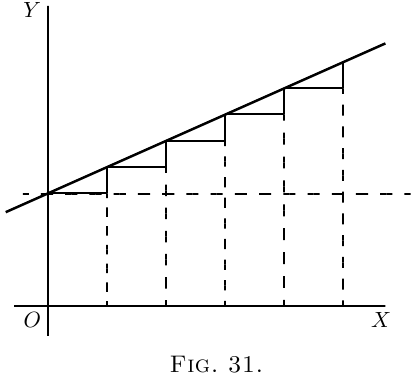
\includegraphics{124a.png}
\end{image}
\begin{image}
\label{Figure32}
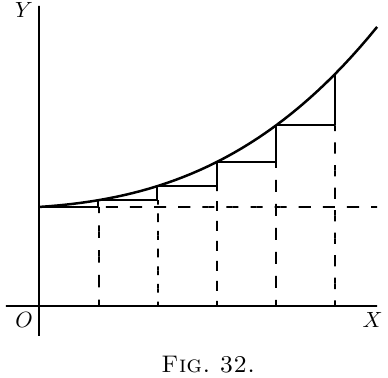
\includegraphics{124b.png}
\end{image}


Suppose a slope constant, as in \ref{Figure31}.
Here, $\dfrac{dy}{dx}$ is of constant value.


Suppose, however, a case in which, like \ref{Figure 32},
the slope itself is getting greater upwards, then
$\dfrac{d\left(\dfrac{dy}{dx}\right)}{dx}$, that is, $\dfrac{d^2y}{dx^2}$, will be \textit{positive}.

\begin{image}
\label{Figure14}
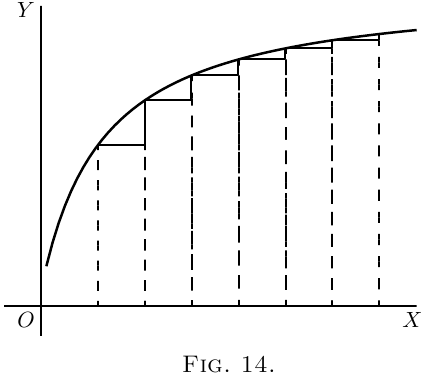
\includegraphics{093a.png}
\end{image}
\begin{image}
\label{Figure33}
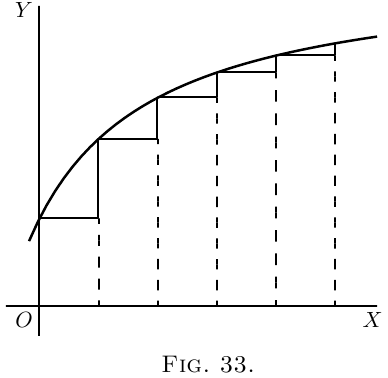
\includegraphics{125a.png}
\end{image}

If the slope is becoming less as you go to the right
(as in /ref{Figure 14}), or as in /ref{Figure 33}, then, even
though the curve may be going upward, since the
change is such as to diminish its slope, its $\dfrac{d^2y}{dx^2}$ will
be \textit{negative}.

It is now time to initiate you into another secret---how
to tell whether the result that you get by ``equating to zero'' is a maximum or a minimum.
The trick is this: After you have differentiated
(so as to get the expression which you equate to
zero), you then differentiate a second time, and look
whether the result of the second differentiation is
\textit{positive} or \textit{negative}. If $\dfrac{d^2y}{dx^2}$ comes out \textit{positive}, then
you know that the value of $y$ which you got was
a \textit{minimum}; but if $\dfrac{d^2y}{dx^2}$ comes out \textit{y}, then

the value of $y$ which you got must be a \textit{maximum}.
That's the rule.

\begin{image}
\label{Figure34}
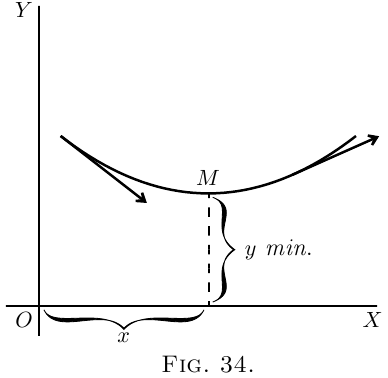
\includegraphics{126a.png}
\end{image}
\begin{image}
\label{Figure35}
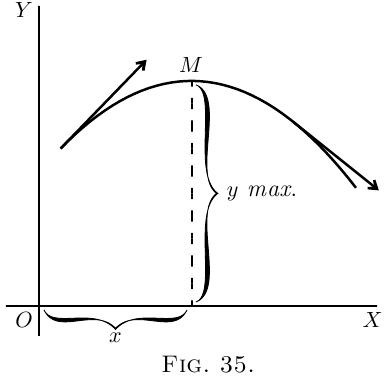
\includegraphics{126b.png}
\end{image}
\begin{image}
\label{Figure15}
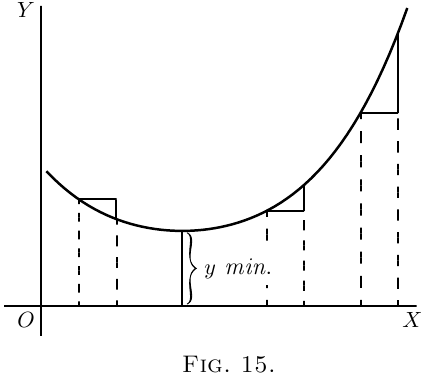
\includegraphics{093b.png}
\end{image}


The reason of it ought to be quite evident. Think
of any curve that has a minimum point in it (like
\ref{Figure 15}, or like \ref{Figure 34}, where the point of
minimum $y$ is marked $M$, and the curve is <em>concave</em>
upwards. To the left of $M$ the slope is downward,
that is, negative, and is getting less negative. To the
right of $M$ the slope has become upward, and is
getting more and more upward. Clearly the change
of slope as the curve passes through $M$ is such that
$\dfrac{d^2y}{dx^2}$ is \textit{positive}, for its operation, as $x$ increases toward
the right, is to convert a downward slope into an
upward one.

\begin{image}
\label{Figure16}
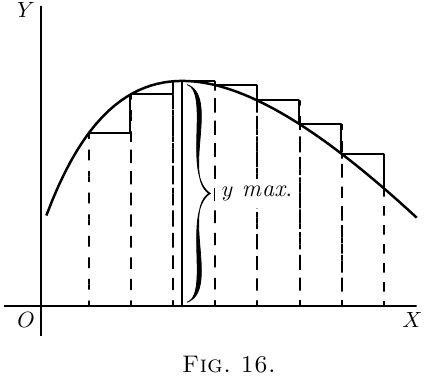
\includegraphics{094a.png}
\end{image}

Similarly, consider any curve that has a maximum
point in it \ref{Figure 16}, or like \ref{Figure 35}, where
the curve is \textit{convex}, and the maximum point is
marked $M$. In this case, as the curve passes through $M$
from left to right, its upward slope is converted

into a downward or negative slope, so that in this
case the ``slope of the slope'' $\dfrac{d^2y}{dx^2}$ is \textit{negative}.

Go back now to the examples of the last chapter
and verify in this way the conclusions arrived at as to
whether in any particular case there is a maximum
or a minimum. You will find below a few worked
out examples.


(1) Find the maximum or minimum of
\begin{align*}
\text{(a)}\quad y &= 4x^2-9x-6; \qquad \text{(b)}\quad y = 6 + 9x-4x^2; \\
\end{align*}

and ascertain if it be a maximum or a minimum in each case.

\begin{align*}
\text{(a)}\quad \dfrac{dy}{dx}
  &= 8x-9=0;\quad x=1\tfrac{1}{8},\quad \text{and } y = -11.065.\\
\dfrac{d^2y}{dx^2}
  &= 8;\quad \text{it is $+$; hence it is a minimum.} \\
\text{(b)}\quad {\dfrac{dy}{dx}}
  &= 9-8x=0;\quad x = 1\tfrac{1}{8};\quad \text{and } y = +11.065.\\
\dfrac{d^2y}{dx^2}
  &= -8;\quad \text{it is $-$; hence it is a maximum.}
\end{align*}

(2) Find the maxima and minima of the function
$y = x^3-3x+16$.
\begin{align*}
\dfrac{dy}{dx}
  &= 3x^2 - 3 = 0;\quad x^2 = 1;\quad \text{and } x = \pm1.\\
\dfrac{d^2y}{dx^2}
  &= 6x;\quad \text{for $x = 1$; it is $+$};
\end{align*}
hence $x=1$ corresponds to a minimum $y=14$. For
$x=-1$ it is $-$; hence $x=-1$ corresponds to a maximum
$y=+18$.


(3) Find the maxima and minima of $y=\dfrac{x-1}{x^2+2}$.
\[
\frac{dy}{dx} = \frac{(x^2+2) \time 1 - (x-1) \times 2x}{(x^2+2)^2}
  = \frac{2x - x^2 + 2}{(x^2 + 2)^2} = 0;
\]
or $x^2 - 2x - 2 = 0$, whose solutions are $x =+2.73$ and
$x=-0.73$.
\begin{align*}
\dfrac{d^2y}{dx^2}
  &= - \frac{(x^2 + 2)^2 \times (2x-2) - (x^2 - 2x - 2)(4x^3 + 8x)}{(x^2 + 2)^4} \\
  &= - \frac{2x^5 - 6x^4 - 8x^3 - 8x^2 - 24x + 8}{(x^2 + 2)^4}.
\end{align*}

The denominator is always positive, so it is sufficient
to ascertain the sign of the numerator.

If we put $x = 2.73$, the numerator is negative; the
maximum, $y = 0.183$.

If we put $x=-0.73$, the numerator is positive; the
minimum, $y=-0.683$.

(4) The expense $C$ of handling the products of a
certain factory varies with the weekly output $P$
according to the relation $C = aP + \dfrac{b}{c+P} + d$, where
$a$, $b$, $c$, $d$ are positive constants. For what output
will the expense be least?
\[
\dfrac{dC}{dP} = a - \frac{b}{(c+P)^2} = 0\quad \text{for maximum or minimum;}
\]
hence $a = \dfrac{b}{(c+P)^2}$ and $P = \pm\sqrt{\dfrac{b}{a}} - c$.

As the output cannot be negative, $P=+\sqrt{\dfrac{b}{a}} - c$.

\begin{align*}
   Now
\frac{d^2C}{dP^2} &= + \frac{b(2c + 2P)}{(c + P)^4},
\end{align*}
which is positive for all the values of $P$; hence
$P = +\sqrt{\dfrac{b}{a}} - c$ corresponds to a minimum.

(5) The total cost per hour $C$ of lighting a building
with $N$ lamps of a certain kind is
\[
C = N\left(\frac{C_l}{t} + \frac{EPC_e}{1000}\right),
\]
where $E$ is the commercial efficiency (watts per candle),

$P$ is the candle power of each lamp,
$t$ is the average life of each lamp in hours,
$C_l =$ cost of renewal in pence per hour of use,
$C_e =$ cost of energy per $1000$ watts per hour.


Moreover, the relation connecting the average life
of a lamp with the commercial efficiency at which it
is run is approximately $t = mE^n$, where $m$ and $n$ are
constants depending on the kind of lamp.

Find the commercial efficiency for which the total
cost of lighting will be least.

\begin{align*}
\text{   We have}\;
C &= N\left(\frac{C_l}{m} E^{-n} + \frac{PC_e}{1000} E\right), \\
\dfrac{dC}{dE}
  &= \frac{PC_e}{1000} - \frac{nC_l}{m} E^{-(n+1)} = 0
\end{align*}
for maximum or minimum.
\[
E^{n+1} = \frac{1000 \times nC_l}{mPC_e}\quad \text{and}\quad
E = \sqrt[n+1]{\frac{1000 \times nC_l}{mPC_e}}.
\]


This is clearly for minimum, since
\[
\frac{d^2C}{dE^2} = (n + 1) \frac{nC_l}{m} E^{-(n+2)},
\]
which is positive for a positive value of $E$.

For a particular type of $16$ candle-power lamps,
$C_l= 17$ pence, $C_e=5$ pence; and it was found that
$m=10$ and $n=3.6$.
\[
E = \sqrt[4.6]{\frac{1000 \times 3.6 \times 17}{10 \times 16 \times 5}}
  = 2.6\text{ watts per candle-power}.
\]


{\Large Exercises\par}(You are advised to plot the graph
of any numerical example.)

\begin{problem}
Find the maxima and minima of
\[
y = x^3 + x^2 - 10x + 8.
\]
= max $x =\answer{-2.19}$, $y = \answer{24.19}$ min $x =\answer{1.52}$, $y =\answer{-1.38}$ 
\end{problem}

\begin{problem}
Given $y = \dfrac{b}{a}x - cx^2$, find expressions for $\dfrac{dy}{dx}$, and
for $\dfrac{d^2y}{dx^2}$, also find the value of $x$ which makes $y$ a
maximum or a minimum, and show whether it is
maximum or minimum. $\dfrac{dy}{dx} = \dfrac{b}{a} - 2cx$; $\dfrac{d^2 y}{dx^2} = -2c$; $x = \dfrac{b}{2ac}$ (\textit{a maximum}).
\end{problem}

\begin{problem}
Find how many maxima and how many minima
there are in the curve, the equation to which is
\[
y = 1 - \frac{x^2}{2} + \frac{x^4}{24};
\]
and how many in that of which the equation is
\[
y = 1 - \frac{x^2}{2} + \frac{x^4}{24} - \frac{x^6}{720}.
\]
(\textit{a}) One maximum and two minima.
(\textit{b}) One maximum. ($x = 0$; other points unreal.)
\end{problem}

\begin{problem}
Find the maxima and minima of
\[
y=2x+1+\frac{5}{x^2}.
\]
Min $x=\answer{1.71}$, $y =\answer{6.14}$
\end{problem}

\begin{problem}
Find the maxima and minima of
\[
y=\frac{3}{x^2+x+1}.
\]
Max $x =\answer{-.5}$, $y =/answer{4}$
\end{problem}

\begin{problem}
Find the maxima and minima of
\[
y=\frac{5x}{2+x^2}.
\]
Max $x = \answer{1.414}$ $y =\answer{1.7675}$ min $x = \answer{-1.414}$, $y = \answer{1.7675}$
\end{problem}

\begin{problem}
Find the maxima and minima of
\[
y=\frac{3x}{x^2-3} + \frac{x}{2} + 5.
\]
Max $x =\answer[tolerance=0.1]{-3.565}$, $y =\answer{2.12}$
Min $x = \answer{3.565}$, $y =\answer{7.88}$
\end{problem}


\begin{problem} Divide a number $N$ into two parts in such a
way that three times the square of one part plus
twice the square of the other part shall be a
minimum.

$\answer{0.4}N$, $\answer{0.6}N$.
\end{problem}

\begin{problem}The efficiency $u$ of an electric generator at
different values of output $x$ is expressed by the
general equation:
\[
u=\frac{x}{a+bx+cx^2};
\]
where $a$ is a constant depending chiefly on the energy
losses in the iron and $c$ a constant depending chiefly
on the resistance of the copper parts. Find an expression
for that value of the output at which the
efficiency will be a maximum.
 $x = \answer{\sqrt{\dfrac{a}{c}}}$.
\end{problem}

(10) Suppose it to be known that consumption of
coal by a certain steamer may be represented by the
formula $y = 0.3 + 0.001v^3$; where $y$ is the number of
tons of coal burned per hour and $v$ is the speed
expressed in nautical miles per hour. The cost of
wages, interest on capital, and depreciation of that
ship are together equal, per hour, to the cost of
$1$ ton of coal. What speed will make the total cost
of a voyage of $1000$ nautical miles a minimum?
And, if coal costs $10$ shillings per ton, what will that
minimum cost of the voyage amount to?

(11) Find the maxima and minima of<a name="ex10"/>
\[
y = \pm\frac{x}{6}\sqrt{x(10-x)}.
\]

(12) Find the maxima and minima of
\[
y= 4x^3 - x^2 - 2x + 1.
\]


(9)  WHAT?

(10)   Speed $8.66$ nautical miles per hour. Time taken $115.47$ hours.
Minimum cost \pounds $112$. $12$ s.

(11)   Max. and min. for $x = 7.5$, $y = \pm5.414$. (See example
no. 10, 

(12)   Min.: $x = \frac{1}{2}$, $y= 0.25$; max.: $x = - \frac{1}{3}$, $y= 1.408$.


\end{document}
